% =====================================================================
%  OPERACIÓN FOGÓN · PHP desde cero · Guía del estudiante
%  Tecnología Web I · UPDS Tarija · FORJA WEB 2026
%  M.Sc. Ing. Juan Pablo Cruz Ovando · jpcruzovando.com
%  Compilar:  lualatex fogon-guia-estudiante.tex   (2 veces, por el índice)
% =====================================================================
\documentclass[11pt]{article}
\usepackage{estilo-jpcruz}
\documento{Operación Fogón · Guía del estudiante}
\usepackage{tocloft}
\usepackage{multicol}
\usetikzlibrary{decorations.pathreplacing,fit,backgrounds,calc}

% ---------------- Tipografía ----------------
\IfFontExistsTF{Fira Sans}{%
  \setmainfont{Fira Sans Light}[BoldFont={Fira Sans SemiBold},ItalicFont={Fira Sans Light Italic},BoldItalicFont={Fira Sans SemiBold Italic}]
  \setsansfont{Fira Sans}[BoldFont={Fira Sans SemiBold}]
  \newfontfamily\titular{Fira Sans Black}
  \newfontfamily\medio{Fira Sans Medium}}{%
  \setmainfont{TeX Gyre Heros}
  \newfontfamily\titular{TeX Gyre Heros}[UprightFont=*-Bold]
  \newfontfamily\medio{TeX Gyre Heros}}
\newfontfamily\simbolos{DejaVu Sans}
\linespread{1.08}

% ---------------- Paleta fuego ----------------
\definecolor{negro}{HTML}{0B0807}
\definecolor{fuego}{HTML}{FF7A18}
\definecolor{brasa}{HTML}{FF3D2E}
\definecolor{oroneon}{HTML}{FFC93C}
\definecolor{cianneon}{HTML}{00E5FF}
\definecolor{verdeneon}{HTML}{39FF88}
\definecolor{lilaneon}{HTML}{B48CFF}
\definecolor{texto}{HTML}{F6ECE4}
\definecolor{grisneon}{HTML}{A8968A}
\definecolor{lineaneon}{HTML}{2E2019}
\definecolor{fuegooscuro}{HTML}{C2530A}

% ---------------- Encabezado y pie ----------------
\fancyhf{}
\renewcommand{\headrulewidth}{0pt}
\renewcommand{\footrulewidth}{0pt}
\newcommand{\seccionactual}{OPERACIÓN FOGÓN · PHP DESDE CERO}
\fancyhead[L]{
\begin{tikzpicture}[overlay]
  \fill[negro] (-0.1,-0.25) rectangle (\headwidth+0.1,0.42);
  \fill[fuego] (-0.1,-0.25) rectangle (0.12,0.42);
  \node[anchor=west,text=fuego,font=\ttfamily\scriptsize] at (0.3,0.08) {// \seccionactual};
  \node[anchor=east,text=grisneon,font=\ttfamily\scriptsize] at (\headwidth-0.15,0.08) {TECNOLOGÍA WEB I · UPDS};
\end{tikzpicture}}
\fancyfoot[L]{\sffamily\scriptsize\color{grisjp}M.Sc. Ing. Juan Pablo Cruz Ovando · jpcruzovando.com}
\fancyfoot[R]{
\begin{tikzpicture}[baseline=-0.6ex]\node[fill=negro,text=fuego,font=\ttfamily\bfseries\scriptsize,rounded corners=1mm,inner sep=3pt]{\thepage};\end{tikzpicture}}

\setcounter{tocdepth}{2}
\renewcommand{\cftsecfont}{\medio\color{fuegooscuro}}
\renewcommand{\cftsecpagefont}{\ttfamily\bfseries\color{fuego}}
\renewcommand{\cftsecleader}{\cftdotfill{\cftdotsep}}
\setlength{\cftbeforesecskip}{0.5em}

% ---------------- Código PHP (oscuro, con colores) ----------------
\lstdefinestyle{phpclaro}{backgroundcolor=\color{negro}, basicstyle=\ttfamily\small\color{texto}, breaklines=true, columns=fullflexible, keepspaces=true,
  showstringspaces=false, upquote=true, aboveskip=0pt, belowskip=0pt,
  numbers=left, numberstyle=\tiny\color{grisneon}, numbersep=6pt,
  alsoletter={\$}, keywordsprefix={\$}, morekeywords=[1]{zzzdummy}, keywordstyle=[1]{\color{cianneon}},
  morekeywords=[2]{echo,if,else,elseif,foreach,as,endforeach,endif,require,function,return,new,try,catch,true,false,count,date,isset,exit,header},
  keywordstyle={[2]\color{fuego}\bfseries},
  morestring=[b]', morestring=[b]", stringstyle=\color{oroneon},
  morecomment=[l]{//}, commentstyle=\color{grisneon}\itshape,
  literate={á}{{á}}1 {é}{{é}}1 {í}{{í}}1 {ó}{{ó}}1 {ú}{{ú}}1 {ñ}{{ñ}}1 {Á}{{Á}}1 {É}{{É}}1 {Ó}{{Ó}}1 {¿}{{¿}}1 {¡}{{¡}}1 {«}{{«}}1 {»}{{»}}1}
\newtcblisting{php}[1]{enhanced, breakable, listing only, colback=negro, colframe=negro, arc=2.5mm, boxrule=0pt,
  left=6mm, right=3mm, top=1.5mm, bottom=1.5mm, drop fuzzy shadow=black!40,
  title={\sffamily\footnotesize\bfseries\color{white}\raisebox{0.5pt}{\tikz{\fill[brasa](0,0)circle(2.2pt);\fill[oroneon](0.22,0)circle(2.2pt);\fill[verdeneon](0.44,0)circle(2.2pt);}}\hspace{2mm}\mdseries\ttfamily #1},
  colbacktitle=negro!85!fuego, coltitle=white, toptitle=1mm, bottomtitle=1mm,
  listing options={style=phpclaro}}
\newtcblisting{salida}[1][lo que ves en el navegador]{enhanced, breakable, listing only, colback=white, colframe=verdejp, arc=2.5mm, boxrule=0.8pt,
  left=3mm, right=3mm, top=1mm, bottom=1mm, title={\sffamily\footnotesize\bfseries #1}, colbacktitle=verdejp, coltitle=white,
  listing options={backgroundcolor=\color{white}, commentstyle=\color{black}, stringstyle=\color{black}, keywordstyle=\color{black}, basicstyle=\ttfamily\small\color{black}, breaklines=true, columns=fullflexible, keepspaces=true, upquote=true,
    literate={á}{{á}}1 {é}{{é}}1 {í}{{í}}1 {ó}{{ó}}1 {ú}{{ú}}1 {ñ}{{ñ}}1 {¡}{{¡}}1 {¿}{{¿}}1}}

% ---------------- Cajas ----------------
\newcommand{\insignia}[2]{\tikz[baseline=-0.7ex]\node[circle,fill=white,text=#1,font=\simbolos\bfseries\footnotesize,inner sep=1.2pt,minimum size=1.15em]{#2};}
\newtcolorbox{analogia}{enhanced, breakable, colback=orojp!8, colframe=orojp, arc=3mm, boxrule=0pt, leftrule=4pt,
  left=3.5mm, drop fuzzy shadow=black!18,
  title={\insignia{orojp}{★}\hspace{1.5mm}\sffamily\bfseries La idea en simple}, colbacktitle=orojp, coltitle=black, fonttitle=\small}
\newtcolorbox{modifica}{enhanced, breakable, colback=cianjp!5, colframe=cianjp, arc=3mm, boxrule=1pt,
  title={\insignia{cianjp}{✎}\hspace{1.5mm}\sffamily\bfseries Modificalo (cambiá, guardá, recargá)}, colbacktitle=cianjp, coltitle=white, fonttitle=\small}
\newtcolorbox{reto}[1][Reto]{enhanced, breakable, colback=rojojp!4, colframe=rojojp!85!black, arc=3mm, boxrule=1pt,
  title={\insignia{rojojp}{⚡}\hspace{1.5mm}\sffamily\bfseries #1}, colbacktitle=rojojp!85!black, coltitle=white, fonttitle=\small, drop fuzzy shadow=black!20}
\newtcolorbox{comprueba}{enhanced, breakable, colback=white, colframe=verdejp, arc=3mm, boxrule=1pt,
  title={\insignia{verdejp}{✓}\hspace{1.5mm}\sffamily\bfseries Comprobá que entendiste \hfill\mdseries\footnotesize respuestas en el Apéndice C},
  colbacktitle=verdejp, coltitle=white, fonttitle=\small}
\newtcolorbox{errores}{enhanced, breakable, colback=negro, colframe=negro, coltext=texto, arc=3mm, boxrule=0pt,
  left=3.5mm, right=3.5mm, borderline west={4pt}{0pt}{brasa}, drop fuzzy shadow=black!30,
  title={\insignia{negro}{!}\hspace{1.5mm}\sffamily\bfseries\color{brasa}ERRORES TÍPICOS DE ESTE NIVEL}, colbacktitle=negro, fonttitle=\small,
  before upper={\color{texto}}}

% Explicación línea por línea
\newenvironment{lineas-explicadas}{\renewcommand{\arraystretch}{1.28}\small
  \begin{longtable}{>{\leavevmode\ttfamily\bfseries\color{fuegooscuro}}p{1.25cm} p{14.0cm}}}{\end{longtable}}

\newcommand{\xp}[1]{\tikz[baseline=-0.65ex]\node[fill=fuego,text=black,rounded corners=1.2mm,font=\sffamily\bfseries\scriptsize,inner sep=2.5pt]{+#1 XP};}
\newcommand{\captura}[2][0.92\linewidth]{\begin{center}\tikz\node[draw=fuego!70,line width=0.8pt,rounded corners=1.5mm,inner sep=0pt]{\includegraphics[width=#1]{#2}};\end{center}}

\newcommand{\parte}[1]{\par\needspace{9\baselineskip}\vspace{3mm}\noindent
  \begin{tikzpicture}
    \fill[negro,rounded corners=1.5mm] (0,0) rectangle (\linewidth,0.72);
    \fill[fuego,rounded corners=1.5mm] (0,0) rectangle (0.2,0.72);
    \node[anchor=west,text=white,font=\medio\normalsize] at (0.45,0.36) {#1};
  \end{tikzpicture}\par\vspace{1.5mm}}

% ---------------- Portadas ----------------
\newcommand{\glitch}[4][west]{%
  \node[anchor=#1,text=brasa,opacity=0.9,font=\titular#3,align=left] at ($(#2)+(-0.08,0.05)$) {#4};
  \node[anchor=#1,text=oroneon,opacity=0.85,font=\titular#3,align=left] at ($(#2)+(0.08,-0.05)$) {#4};
  \node[anchor=#1,text=white,font=\titular#3,align=left] at (#2) {#4};}
\newcommand{\glitchancho}[3]{%
  \node[anchor=south west,text=brasa,opacity=0.9,font=\titular#2,text width=16.6cm,align=left] at ($(#1)+(-0.08,0.05)$) {\hyphenpenalty=10000 #3};
  \node[anchor=south west,text=oroneon,opacity=0.85,font=\titular#2,text width=16.6cm,align=left] at ($(#1)+(0.08,-0.05)$) {\hyphenpenalty=10000 #3};
  \node[anchor=south west,text=white,font=\titular#2,text width=16.6cm,align=left] at (#1) {\hyphenpenalty=10000 #3};}
\newcommand{\fondofuego}{%
  \fill[negro] (current page.south west) rectangle (current page.north east);
  \shade[top color=negro,bottom color=fuego!35!negro] ($(current page.south west)+(0,0)$) rectangle ($(current page.south east)+(0,7)$);
  \foreach \x in {0,1,...,21}{\draw[lineaneon,line width=0.3pt,opacity=0.7] ($(current page.south west)+(\x,0)$) -- ++(0,29.7);}
  \foreach \y in {0,1,...,30}{\draw[lineaneon,line width=0.3pt,opacity=0.7] ($(current page.south west)+(0,\y)$) -- ++(21,0);}}

% \nivelportada{num}{titulo}{color}{frase}{tiempo}{xp}
\newcommand{\nivelportada}[6]{%
  \clearpage\thispagestyle{empty}\phantomsection\addcontentsline{toc}{section}{Nivel #1 · #2}%
  \renewcommand{\seccionactual}{NIVEL #1 · #2}%
  \begin{tikzpicture}[remember picture,overlay]
    \fondofuego
    \coordinate (R) at ($(current page.north east)+(-5.2,-7.6)$);
    \foreach \r in {1.2,2.4,3.6,4.8,6.0}{\draw[#3,opacity=0.3,line width=0.6pt] (R) circle (\r);}
    \fill[#3,opacity=0.15] (R) -- ++(15:6) arc (15:75:6) -- cycle;
    \draw[#3,line width=1.6pt] (R) -- ++(75:6);
    \node[text=#3,opacity=0.18,font=\titular\fontsize{230}{230}\selectfont] at ($(R)+(0.2,-0.4)$) {#1};
    \node[anchor=west,text=#3,font=\ttfamily\large] at ($(current page.west)+(2,3.5)$) {> NIVEL #1 · ENCENDIENDO EL FUEGO};
    \coordinate (T) at ($(current page.west)+(1.95,-0.6)$);
    \glitchancho{T}{\fontsize{38}{42}\selectfont}{#2}
    \node[anchor=north west,text=texto,font=\Large\itshape,text width=15.5cm] at ($(current page.west)+(2,-1.6)$) {#4};
    \node[anchor=west,draw=#3,text=#3,font=\ttfamily\small,rounded corners=1.5mm,inner sep=4pt] (c1) at ($(current page.west)+(2,-3.75)$) {TIEMPO #5};
    \node[anchor=west,fill=#3,text=black,font=\ttfamily\bfseries\small,rounded corners=1.5mm,inner sep=4pt] at ($(c1.east)+(0.3,0)$) {+#6 XP};
    \node[anchor=north west,text=grisneon,font=\ttfamily\small] at ($(current page.south west)+(2,8.4)$) {EN ESTE NIVEL};
    \foreach \i/\t in {1/La idea en simple,2/Míralo funcionar,3/El código explicado línea por línea}{
      \node[anchor=west,text=texto,font=\small] at ($(current page.south west)+(2,{7.9-0.62*\i})$) {\textcolor{#3}{\ttfamily 0\i}\quad \t};}
    \foreach \i/\t in {4/Modificalo,5/El reto,6/Errores típicos · Comprobá}{
      \node[anchor=west,text=texto,font=\small] at ($(current page.south west)+(10.5,{7.9-0.62*(\i-3)})$) {\textcolor{#3}{\ttfamily 0\i}\quad \t};}
    \node[anchor=south west,text=grisneon,font=\ttfamily\scriptsize] at ($(current page.south west)+(2,1.2)$) {OPERACIÓN FOGÓN · PHP DESDE CERO · TECNOLOGÍA WEB I · UPDS TARIJA};
  \end{tikzpicture}
  \clearpage}

\begin{document}

% ============================ PORTADA ============================
\thispagestyle{empty}

\begin{tikzpicture}[remember picture,overlay]
  \fondofuego
  \coordinate (R) at ($(current page.center)+(3.2,4.4)$);
  \foreach \r in {1.2,2.4,3.6,4.8,6.0,7.2,8.4}{\draw[fuego,opacity=0.22,line width=0.6pt] (R) circle (\r);}
  \fill[fuego,opacity=0.13] (R) -- ++(20:8.4) arc (20:78:8.4) -- cycle;
  \draw[oroneon,line width=1.6pt] (R) -- ++(78:8.4);
  \foreach \x/\y/\c/\t in {1.6/3.4/oroneon/echo,3.9/1.2/cianneon/\$variable,-2.6/2.4/verdeneon/foreach,-1.8/-2.9/brasa/\$\_POST,2.9/-2.6/lilaneon/PDO,-4.3/-0.6/fuego/if,0.6/5.6/oroneon/MySQL,5.6/-0.6/cianneon/<?php}{
    \fill[\c] ($(R)+(\x,\y)$) circle (3.2pt);
    \node[text=\c,font=\ttfamily\small,anchor=west] at ($(R)+(\x,\y)+(0.15,0)$) {\t};}
  \node[anchor=west,text=fuego,font=\ttfamily\large] at ($(current page.south west)+(2,11.6)$) {Tecnología Web I · FORJA WEB 2026 · Guía del estudiante};
  \coordinate (T1) at ($(current page.south west)+(1.95,10.0)$); \glitch{T1}{\fontsize{56}{60}\selectfont}{OPERACIÓN}
  \coordinate (T2) at ($(current page.south west)+(1.95,8.0)$);  \glitch{T2}{\fontsize{56}{60}\selectfont}{FOGÓN}
  \node[anchor=west,text=texto,font=\LARGE] at ($(current page.south west)+(2,6.4)$) {PHP desde cero: hoy el cocinero entra a la cocina};
  \node[anchor=north west,text=texto!80,font=\normalsize,text width=16.5cm] at ($(current page.south west)+(2,5.6)$)
    {Para quienes \textbf{nunca} vieron PHP. Cada nivel trae: la idea en simple, el ejemplo funcionando, el código explicado
     línea por línea, algo para modificar, un reto, los errores típicos y preguntas para comprobar que entendiste.};
  \node[anchor=south west,text=grisneon,font=\small] at ($(current page.south west)+(2,2.1)$) {M.Sc. Ing. Juan Pablo Cruz Ovando · UPDS Tarija · Noviembre 2026};
  \node[anchor=south west,text=grisneon,font=\scriptsize] at ($(current page.south west)+(2,1.5)$) {70213044 / 61865265 · gerencia@jpcruzovando.com · jpcruzovando.com};
  \IfFileExists{imagenes/danko.png}{\node[anchor=north east] at ($(current page.north east)+(-1,-1)$) {\includegraphics[height=1.5cm]{imagenes/danko.png}};}{}
\end{tikzpicture}
\clearpage

\setcounter{page}{2}
\renewcommand{\contentsname}{\titular\color{fuegooscuro}Contenido}
\tableofcontents

% =====================================================================
%  INTRODUCCIÓN · cómo usar la guía, la cocina de la web, el laboratorio
% =====================================================================
\clearpage
\renewcommand{\seccionactual}{CÓMO USAR ESTA GUÍA}
\section*{Cómo usar esta guía}
\addcontentsline{toc}{section}{Cómo usar esta guía}

Hoy vas a aprender \textbf{PHP desde cero}, aunque nunca hayas escrito una línea de código de servidor. La clase está
armada como un juego: \textbf{7 niveles}, cada uno con su desafío y sus puntos de experiencia (XP).

\subsection*{Cada nivel tiene siempre las mismas partes}
\renewcommand{\arraystretch}{1.1}
\begin{tabularx}{\linewidth}{>{\leavevmode\sffamily\bfseries\color{fuegooscuro}}p{4.6cm} X}
  La idea en simple & Una comparación con la vida real. Si solo leés una cosa, que sea esta. \\
  Míralo funcionar & Abrís la página en el navegador y ves el resultado. \\
  El código explicado & El archivo, \textbf{línea por línea}, en castellano. \\
  Modificalo & Cambiás cosas pequeñas y ves qué pasa. Así se aprende de verdad. \\
  El reto & Escribís algo vos. La solución está en la carpeta \texttt{soluciones}, pero \textbf{intentá antes}. \\
  Errores típicos & Lo que le pasa a todo el mundo, y cómo arreglarlo. \\
  Comprobá que entendiste & Preguntas cortas. Las respuestas están en el Apéndice C. \\
\end{tabularx}

\subsection*{El método: ver $\rightarrow$ modificar $\rightarrow$ crear}
\begin{center}
\begin{tikzpicture}[font=\sffamily\small]
  \node[draw=cianjp,fill=cianjp!8,rounded corners=2mm,line width=1pt,minimum width=4.4cm,minimum height=1.5cm,align=center] (a) at (0,0) {\textbf{1 · VER}\\el ejemplo funcionando};
  \node[draw=orojp,fill=orojp!10,rounded corners=2mm,line width=1pt,minimum width=4.4cm,minimum height=1.5cm,align=center] (b) at (5.4,0) {\textbf{2 · MODIFICAR}\\cambiar una línea y ver qué pasa};
  \node[draw=rojojp,fill=rojojp!8,rounded corners=2mm,line width=1pt,minimum width=4.4cm,minimum height=1.5cm,align=center] (c) at (10.8,0) {\textbf{3 · CREAR}\\escribir algo propio};
  \draw[-{Stealth},thick,grisjp] (a) -- (b); \draw[-{Stealth},thick,grisjp] (b) -- (c);
\end{tikzpicture}
\end{center}

\subsection*{Tu rango de cocinero}
\renewcommand{\arraystretch}{1.05}
\begin{tabularx}{\linewidth}{l X >{\bfseries}l}
\toprule
\textbf{Nivel} & \textbf{Qué aprendés} & XP \\
\midrule
0 · El gancho & Por qué existe PHP y dónde se ejecuta & 50 \\
1 · Hablar & \texttt{echo}, variables, comillas & 100 \\
2 · Decidir y repetir & \texttt{if}, arrays, \texttt{foreach} & 150 \\
3 · Escuchar & Formularios con \texttt{\$\_GET} y \texttt{\$\_POST} & 150 \\
4 · Recordar & PHP + MySQL con PDO & 200 \\
5 · El museo & Los 5 errores que todos cometen & 100 \\
X · Jefe final & PHP en tu proyecto FORJA WEB & 250 \\
\midrule
 & \textbf{Total} & 1000 \\
\bottomrule
\end{tabularx}
\vspace{1mm}

\begin{center}
\begin{tikzpicture}[font=\sffamily\small]
  \foreach \i/\c/\t/\r in {0/grisjp/Ayudante de cocina/0--299,1/orojp/Cocinero/300--599,2/fuego/Chef/600--899,3/rojojp/Chef ejecutivo/900--1000}{
    \node[draw=\c,fill=\c!10,rounded corners=2mm,line width=1pt,minimum width=3.7cm,minimum height=1.3cm,align=center] at ({\i*4.05},0) {\textbf{\t}\\\texttt{\r} XP};}
\end{tikzpicture}
\end{center}

% =====================================================================
\clearpage
\renewcommand{\seccionactual}{LA COCINA DE LA WEB}
\section*{La cocina de la web}
\addcontentsline{toc}{section}{La cocina de la web}

\subsection*{HTML muestra. PHP piensa.}
Hasta ahora hiciste páginas con \textbf{HTML}: dicen \textbf{siempre lo mismo}. Si escribís «Son las 10:00», dice
«Son las 10:00» aunque sean las tres de la tarde. HTML sabe \emph{mostrar}, pero no sabe \emph{pensar}.

\textbf{PHP} es un lenguaje de programación que corre \textbf{en el servidor}. Antes de mandarte la página, PHP puede
calcular la hora, decidir qué saludo poner, leer datos de una base de datos, recibir lo que escribiste en un
formulario\ldots\ y recién entonces \textbf{arma el HTML} y te lo envía.

\begin{analogia}
Pensá en un restaurante. Vos (el \textbf{navegador}) le pedís un plato al \textbf{mozo} (\textbf{Apache}, el servidor web).
Si pedís algo ya hecho, como una gaseosa (un archivo \texttt{.html}), el mozo te lo trae tal cual. Si pedís algo que hay
que cocinar (un archivo \texttt{.php}), el mozo se lo pasa al \textbf{cocinero} (\textbf{PHP}), que busca ingredientes en la
\textbf{despensa} (\textbf{MySQL}), cocina y le entrega el plato terminado al mozo. \textbf{Vos nunca entrás a la cocina}:
solo ves el plato servido (el HTML).
\end{analogia}

\begin{center}
\begin{tikzpicture}[font=\sffamily\small,
  c/.style={draw=#1,fill=#1!8,rounded corners=2mm,line width=1pt,minimum width=3.1cm,minimum height=1.45cm,align=center}]
  \node[c=grisjp] (n) at (0,0) {\textbf{Navegador}\\(el cliente)};
  \node[c=cianjp] (a) at (4.4,0) {\textbf{Apache}\\(el mozo)};
  \node[c=fuego] (p) at (8.8,0) {\textbf{PHP}\\(el cocinero)};
  \node[c=lilaneon!80!black] (m) at (13.2,0) {\textbf{MySQL}\\(la despensa)};
  \draw[-{Stealth},thick,grisjp] (n.north east) to[bend left=18] node[above,font=\scriptsize]{pide \texttt{hora.php}} (a.north west);
  \draw[-{Stealth},thick,cianjp] (a.north east) to[bend left=18] node[above,font=\scriptsize]{«cociná esto»} (p.north west);
  \draw[-{Stealth},thick,lilaneon!80!black] (p.north east) to[bend left=18] node[above,font=\scriptsize]{pide datos} (m.north west);
  \draw[-{Stealth},thick,verdejp] (p.south west) to[bend left=18] node[below,font=\scriptsize]{HTML terminado} (a.south east);
  \draw[-{Stealth},thick,verdejp] (a.south west) to[bend left=18] node[below,font=\scriptsize]{la página} (n.south east);
\end{tikzpicture}
\end{center}

\subsection*{La idea más importante del día}
\begin{marco}[fuego]{PHP se ejecuta en el SERVIDOR}
El navegador \textbf{nunca} ve tu código PHP. Solo recibe el \textbf{resultado}: HTML. Por eso PHP puede guardar
secretos (como la contraseña de la base de datos) que nadie desde afuera puede leer.
\end{marco}

\subsection*{¿Por qué PHP?}
\begin{itemize}
  \item Según W3Techs (agosto de 2026), PHP se usa en alrededor del \textbf{70\,\%} de los sitios web cuyo lenguaje de servidor se conoce: \textbf{7 de cada 10}.
  \item \textbf{WordPress}, con el que se hacen muchísimos blogs, tiendas y sitios de empresas, está hecho en PHP.
  \item Es de los más fáciles para empezar: hoy, en tres horas, vas a guardar datos en una base de datos.
\end{itemize}

% =====================================================================
\clearpage
\renewcommand{\seccionactual}{ENCENDER LA COCINA}
\section*{Encender la cocina (tu laboratorio)}
\addcontentsline{toc}{section}{Encender la cocina (tu laboratorio)}

Todo corre en \textbf{Docker}, así que no tenés que instalar XAMPP ni configurar nada.
El laboratorio tiene \textbf{tres contenedores}:

\renewcommand{\arraystretch}{1.3}
\begin{tabularx}{\linewidth}{>{\ttfamily\bfseries}l l X}
\toprule
\normalfont\bfseries Contenedor & \textbf{Qué es} & \textbf{Dónde lo ves} \\
\midrule
fogon-web & Apache + PHP 8.3 (mozo y cocinero) & \texttt{http://localhost:8090} \\
fogon-db  & MySQL 8.4 (la despensa) & \texttt{127.0.0.1:3308} (Workbench) \\
fogon-pma & phpMyAdmin (la ventana a la despensa) & \texttt{http://localhost:8091} \\
\bottomrule
\end{tabularx}

\parte{Paso 1 · Requisitos}
\begin{itemize}
  \item \textbf{Docker Desktop} abierto (la ballena tiene que estar quieta, no animada).
  \item \textbf{VS Code} (o cualquier editor de texto; el Bloc de notas también sirve).
  \item La carpeta \texttt{operacion-fogon} que comparte el profe, copiada en tu Escritorio.
\end{itemize}

\parte{Paso 2 · Encender}
Abrí la carpeta \texttt{operacion-fogon}, hacé \textbf{clic derecho en un espacio vacío $\rightarrow$ Abrir en Terminal} y escribí:
\begin{terminal}[PowerShell]{la primera vez tarda unos minutos (descarga imágenes)}
Set-ExecutionPolicy -Scope Process Bypass
.\scripts\iniciar.ps1
\end{terminal}
El script levanta todo, espera a que MySQL esté listo y abre el navegador en \texttt{http://localhost:8090}.
Tenés que ver el \textbf{mapa de la cocina} con el cocinero y la despensa \textbf{encendidos}.

\captura[0.85\linewidth]{imagenes/index.png}

\parte{Paso 3 · Abrir tus recetas en VS Code}
En VS Code: \textbf{Archivo $\rightarrow$ Abrir carpeta} $\rightarrow$ elegí la carpeta \texttt{operacion-fogon}. Tus archivos
están dentro de \texttt{www}:
\begin{terminal}[estructura]{carpeta operacion-fogon}
www/
  00-gancho/       nivel 0: HTML vs PHP
  01-hablar/       nivel 1: echo y variables
  02-decidir/      nivel 2: if, arrays, foreach
  03-escuchar/     nivel 3: formularios GET y POST
  04-recordar/     nivel 4: PHP + MySQL
  05-errores/      el museo de los 5 errores
  06-reto-final/   jefe final: formulario de contacto
  soluciones/      soluciones de los retos
db/init.sql        la despensa: tablas y datos iniciales
docker-compose.yml el plano de la cocina
\end{terminal}

\parte{Paso 4 · El ciclo que vas a repetir 100 veces}
\begin{center}
\begin{tikzpicture}[font=\sffamily\small,
  c/.style={draw=#1,fill=#1!8,rounded corners=2mm,line width=1pt,minimum width=3.6cm,minimum height=1.3cm,align=center}]
  \node[c=cianjp] (a) at (0,0) {\textbf{1 · Editás}\\en VS Code};
  \node[c=orojp] (b) at (4.8,0) {\textbf{2 · Guardás}\\\texttt{Ctrl + S}};
  \node[c=fuego] (c) at (9.6,0) {\textbf{3 · Recargás}\\\texttt{F5} en el navegador};
  \draw[-{Stealth},thick,grisjp] (a) -- (b); \draw[-{Stealth},thick,grisjp] (b) -- (c);
  \draw[-{Stealth},thick,verdejp] (c.south) to[bend left=22] node[below,font=\scriptsize]{y otra vez} (a.south);
\end{tikzpicture}
\end{center}
No hace falta reiniciar nada: la carpeta \texttt{www} está «conectada» al contenedor. Guardás y el servidor ya tiene el cambio.

\begin{ojo}[Si algo no anda]
\textbf{El puerto está ocupado} (8090, 8091 o 3308): en \texttt{docker-compose.yml} cambiá el número de la \emph{izquierda}, por ejemplo \texttt{"8095:80"}.
\textbf{«La despensa está cerrada»}: MySQL tarda unos segundos la primera vez; esperá y recargá.
\textbf{Docker no funciona en tu PC}: usá el plan B, \texttt{.\textbackslash scripts\textbackslash plan-b-sin-base.ps1}, que levanta solo PHP y alcanza para los niveles 0 a 3 y el museo.
\end{ojo}

% =====================================================================
%  LOS NIVELES
% =====================================================================

% =====================================================================
\nivelportada{0}{El gancho: HTML no sabe qué hora es}{oroneon}{Dos páginas idénticas. Una dice lo mismo para siempre. La otra piensa.}{15 min}{50}

\begin{analogia}
Una página \textbf{HTML} es como un \textbf{cartel impreso}: dice «Buenos días» aunque sean las nueve de la noche.
Una página \textbf{PHP} es como un \textbf{recepcionista}: mira el reloj antes de saludarte.
\end{analogia}

\parte{Míralo funcionar}
Abrí \texttt{http://localhost:8090/00-gancho/} y entrá a los dos archivos. \textbf{Recargá cada uno 5 veces} (F5).

\begin{center}
\begin{minipage}{0.48\linewidth}\centering{\small\bfseries hora.html}\\[1mm]\tikz\node[draw=grisjp,rounded corners=1mm,inner sep=0pt]{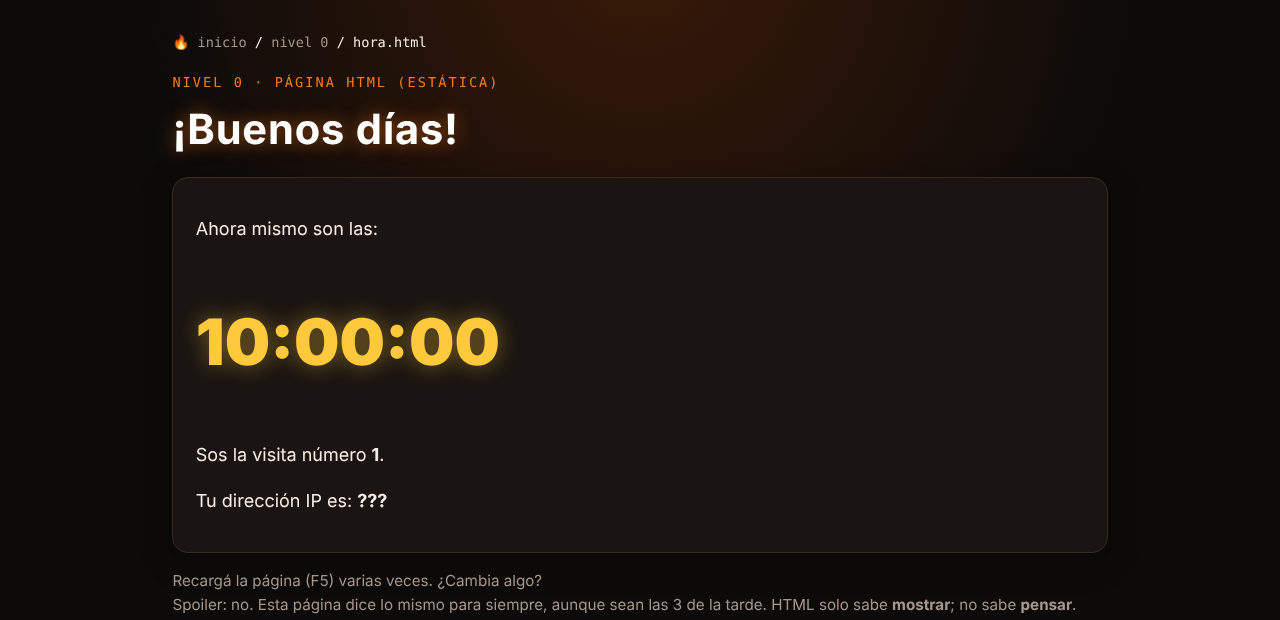
\includegraphics[width=\linewidth]{imagenes/hora-html.png}};\end{minipage}\hfill
\begin{minipage}{0.48\linewidth}\centering{\small\bfseries\color{fuego} hora.php}\\[1mm]\tikz\node[draw=fuego,rounded corners=1mm,inner sep=0pt]{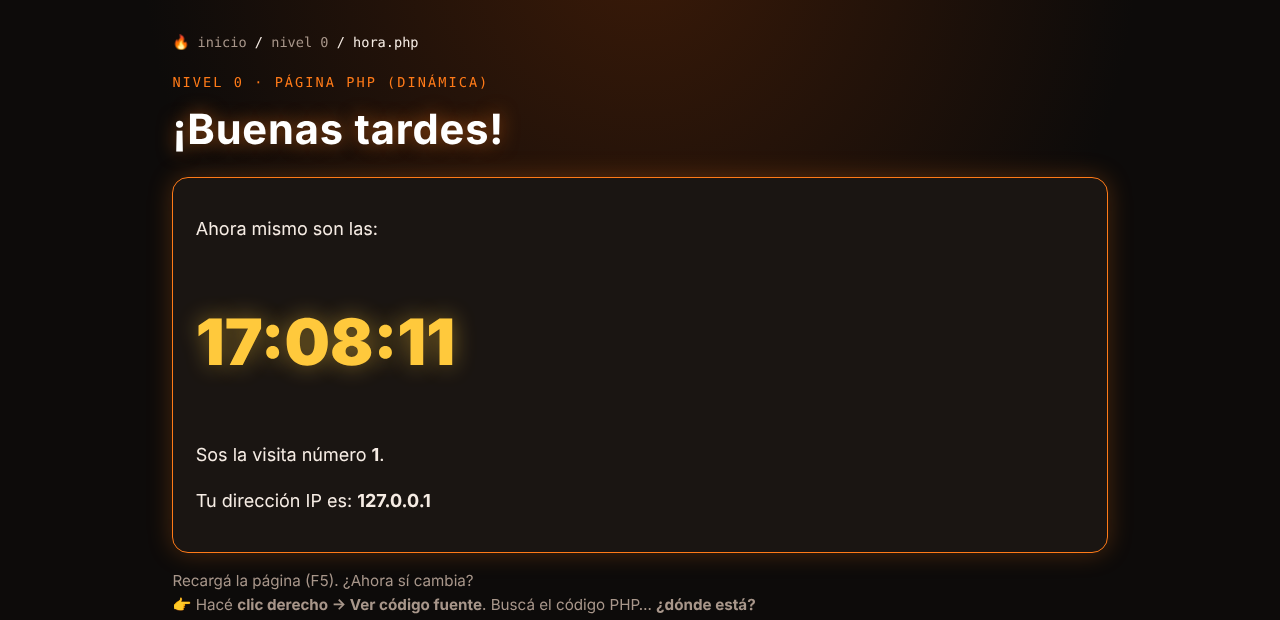
\includegraphics[width=\linewidth]{imagenes/hora-php.png}};\end{minipage}
\end{center}
La página HTML dice \textbf{10:00:00} y «visita número 1» para siempre. La PHP cambia la hora, cuenta tus visitas,
te saluda según el momento del día y sabe tu dirección IP.

\parte{El experimento clave: ver el código fuente}
En \texttt{hora.php}, hacé \textbf{clic derecho $\rightarrow$ Ver código fuente} (o \texttt{Ctrl+U}). Buscá el código PHP\ldots\ \textbf{no está}.
\begin{salida}[lo que recibe el navegador (resumido)]
<h1>¡Buenas tardes!</h1>
<p class="enorme">17:08:11</p>
<p>Sos la visita número <b>3</b>.</p>
\end{salida}
El navegador solo recibió \textbf{el resultado}. El código se ejecutó en el servidor, adentro del contenedor \texttt{fogon-web}.

\parte{El código explicado}
\begin{php}{www/00-gancho/hora.php (la parte PHP)}
<?php
session_start();

$hora = (int) date('H');

if ($hora < 12) {
    $saludo = '¡Buenos días!';
} elseif ($hora < 19) {
    $saludo = '¡Buenas tardes!';
} else {
    $saludo = '¡Buenas noches!';
}

$_SESSION['visitas'] = ($_SESSION['visitas'] ?? 0) + 1;
$ip = $_SERVER['REMOTE_ADDR'];
?>
<h1><?php echo $saludo; ?></h1>
\end{php}
\begin{lineas-explicadas}
1 & \texttt{<?php} abre la «zona PHP». Todo lo que sigue es código que ejecuta el servidor. \\
2 & \texttt{session\_start()} le da a PHP una «memoria» por visitante: así puede contar tus visitas. \\
4 & \texttt{date('H')} pregunta la hora actual (de 0 a 23) y la guarda en la variable \texttt{\$hora}. \\
6--12 & \texttt{if / elseif / else}: según la hora, elige un saludo distinto. (Lo vemos en el nivel 2.) \\
14 & Suma 1 a tus visitas. El \texttt{?? 0} significa «si todavía no había visitas, empezá en 0». \\
15 & \texttt{\$\_SERVER['REMOTE\_ADDR']} es la dirección IP de quien visita la página. \\
16 & \texttt{?>} cierra la zona PHP. Lo que sigue es HTML normal. \\
17 & \texttt{echo} escribe el saludo \textbf{dentro} del HTML. \\
\end{lineas-explicadas}

\begin{comprueba}
\begin{enumerate}
  \item ¿Por qué al ver el código fuente de \texttt{hora.php} no aparece el código PHP?
  \item Si mirás \texttt{hora.php} a las 20:30, ¿qué saludo sale?
  \item ¿Puede alguien que visita tu página leer la contraseña de tu base de datos escrita en un archivo PHP? ¿Por qué?
\end{enumerate}
\end{comprueba}

% =====================================================================
\nivelportada{1}{Hablar: echo y variables}{cianneon}{PHP escribe HTML por vos. Primero, a hablar.}{25 min}{100}

\begin{analogia}
Una \textbf{variable} es una \textbf{cajita con una etiqueta}. En la etiqueta escribís un nombre (\texttt{\$nombre}) y adentro
guardás algo (\texttt{'Ana'}). Cuando necesitás el dato, pedís la cajita por su nombre.
\texttt{echo} es la \textbf{boca} de PHP: lo que le das, lo escribe en la página.
\end{analogia}

\parte{Míralo funcionar}
Abrí en el navegador \texttt{http://localhost:8090/01-hablar/1-echo.php}\\ y, al mismo tiempo, el archivo \texttt{www/01-hablar/1-echo.php} en VS Code.
\captura[0.8\linewidth]{imagenes/echo.png}

\parte{El código explicado}
\begin{php}{www/01-hablar/1-echo.php (resumido)}
<?php
$nombre  = 'Juan Pablo';
$materia = 'Tecnología Web I';
$anio    = 2026;
$precio  = 12.50;
?>
<p>Hola, soy <?php echo $nombre; ?>.</p>
<p><?php echo 'Estudio ' . $materia . ' en el año ' . $anio; ?></p>
<p><?php echo "El cafecito cuesta $precio bolivianos."; ?></p>
<p><?php echo 'Con comillas simples sale: $precio'; ?></p>
<p>Tres cafecitos: <?php echo $precio * 3; ?> Bs.</p>
<p><?= strtoupper($nombre) ?></p>
\end{php}
\begin{lineas-explicadas}
2--5 & Cuatro variables. Todas empiezan con \texttt{\$}. Los \textbf{textos} van entre comillas; los \textbf{números}, sin comillas. Cada línea termina con \texttt{;}. \\
7 & \texttt{echo \$nombre;} escribe el contenido de la cajita \texttt{\$nombre} dentro del párrafo. \\
8 & El \textbf{punto} (\texttt{.}) \textbf{pega} textos: «Estudio » + «Tecnología Web I» + « en el año » + 2026. \\
9 & Con comillas \textbf{dobles}, PHP busca variables adentro y las \textbf{reemplaza} por su valor. \\
10 & Con comillas \textbf{simples}, PHP \textbf{no} reemplaza: sale el texto \texttt{\$precio} tal cual. \\
11 & PHP hace cuentas: \texttt{*} multiplica, \texttt{+} suma, \texttt{-} resta, \texttt{/} divide. \\
12 & \texttt{<?= ... ?>} es un \textbf{atajo} de \texttt{<?php echo ... ?>}. \texttt{strtoupper} pasa a mayúsculas: PHP trae miles de funciones así. \\
\end{lineas-explicadas}

\begin{salida}
Hola, soy Juan Pablo.
Estudio Tecnología Web I en el año 2026
El cafecito cuesta 12.5 bolivianos.
Con comillas simples sale: $precio
Tres cafecitos: 37.5 Bs.
JUAN PABLO
\end{salida}

\begin{modifica}
\begin{enumerate}
  \item Cambiá \texttt{\$nombre} por tu nombre. Guardá (\texttt{Ctrl+S}) y recargá (\texttt{F5}). \xp{10}
  \item Cambiá el precio a \texttt{15}. ¿Qué pasa con el total de tres cafecitos? \xp{10}
  \item Agregá \texttt{\$ciudad = 'Tarija';} y mostrala en un párrafo nuevo con comillas dobles. \xp{10}
  \item Probá \texttt{strtolower} y \texttt{strlen(\$nombre)}. ¿Qué hace cada una? \xp{10}
\end{enumerate}
\end{modifica}

\parte{El reto: tu tarjeta de presentación viva}
Abrí \texttt{www/01-hablar/2-tarjeta.php}. PHP ya calcula tu edad y los días que faltan para la defensa del proyecto:
\begin{php}{lo que PHP calcula solo}
$anioActual = (int) date('Y');
$edad       = $anioActual - $anioNacimiento;

$defensa = strtotime('2026-11-25');
$dias    = (int) ceil(($defensa - time()) / 86400);
\end{php}
\begin{lineas-explicadas}
1 & \texttt{date('Y')} da el año actual. El \texttt{(int)} lo convierte en número entero. \\
2 & Una resta: tu edad (aproximada) sale sola cada año. \\
4 & \texttt{strtotime} convierte una fecha en \textbf{segundos} (así mide PHP el tiempo). \\
5 & Fecha de la defensa menos ahora (\texttt{time()}) $=$ segundos que faltan. Dividido \texttt{86400} (los segundos de un día) $=$ días. \texttt{ceil} redondea hacia arriba. \\
\end{lineas-explicadas}

\begin{reto}[Reto · tu tarjeta \xp{60}]
\begin{enumerate}
  \item \textbf{TODO 1:} poné tus datos reales (nombre, carrera, año de nacimiento, frase).
  \item \textbf{TODO 2:} creá una variable \texttt{\$color} con un color en inglés (\texttt{'orange'}, \texttt{'deepskyblue'}, \texttt{'lime'}\ldots).
  \item \textbf{TODO 3:} usala en el borde de la tarjeta: cambiá \texttt{border-color: orange} por \texttt{border-color: <?= \$color ?>}.
  \item \textbf{Bonus:} si faltan 1 o menos días, que diga «¡Es mañana!». (Vas a necesitar un \texttt{if}: espiá el nivel 2.)
\end{enumerate}
Solución: \texttt{http://localhost:8090/soluciones/2-tarjeta-solucion.php}
\end{reto}

\begin{errores}
\textbf{Pantalla con «Parse error»}: casi siempre falta un \texttt{;} al final de la línea \emph{anterior} a la que dice PHP.\\[1mm]
\textbf{Sale \texttt{\$nombre} escrito tal cual}: usaste comillas simples. Cambiá a dobles o usá el punto.\\[1mm]
\textbf{«Undefined variable»}: escribiste mal el nombre. \texttt{\$Nombre} y \texttt{\$nombre} son \textbf{distintas}.
\end{errores}

\begin{comprueba}
\begin{enumerate}
  \item ¿Con qué símbolo empiezan todas las variables en PHP?
  \item ¿Qué muestra \texttt{echo 'Total: \$precio';}? ¿Y \texttt{echo "Total: \$precio";}?
  \item ¿Para qué sirve el punto (\texttt{.}) en \texttt{'Hola, ' . \$nombre}?
  \item ¿Qué es \texttt{<?= \$x ?>}?
\end{enumerate}
\end{comprueba}

% =====================================================================
\nivelportada{2}{Decidir y repetir: if, arrays y foreach}{fuego}{El código toma decisiones… y hace el trabajo repetitivo por vos.}{30 min}{150}

\begin{analogia}
\textbf{if} es el \textbf{portero} de un boliche: mira tu edad y decide si pasás. Un \textbf{array} es una \textbf{lista}
(como la lista de compras) o una \textbf{ficha} (nombre: Saice, precio: 38). \textbf{foreach} es el \textbf{mozo que recorre todas las
mesas}: hace lo mismo con cada una, sin que tengas que escribirlo diez veces.
\end{analogia}

\parte{Parte A · Decidir con if}
Abrí \texttt{www/02-decidir/1-edad.php}:
\begin{php}{www/02-decidir/1-edad.php (resumido)}
$edad = 17;

if ($edad < 13) {
    $mensaje = 'Sos un niño: menú infantil';
} elseif ($edad < 18) {
    $mensaje = 'Sos adolescente: nada de bebidas para adultos';
} elseif ($edad < 60) {
    $mensaje = 'Sos adulto: acceso completo';
} else {
    $mensaje = 'Adulto mayor: 20 % de descuento';
}
\end{php}
\begin{lineas-explicadas}
3 & \texttt{if (condición) \{ ... \}}: si la condición es verdadera, se ejecuta lo que está entre llaves. \\
5 & \texttt{elseif}: «si no se cumplió lo anterior, probá esto». Se pueden poner varios. \\
9 & \texttt{else}: «en cualquier otro caso». No lleva condición. \\
-- & \textbf{Clave}: PHP prueba de arriba hacia abajo y se queda con la \textbf{primera} condición verdadera. Las demás se ignoran. \\
\end{lineas-explicadas}

\begin{marco}[fuego]{Para comparar}
\renewcommand{\arraystretch}{1.2}
\begin{tabularx}{\linewidth}{>{\ttfamily\bfseries}l X >{\ttfamily\bfseries}l X}
<  & menor & ==  & igual (¡dos signos!) \\
>  & mayor & !=  & distinto \\
<= & menor o igual & \&\& & «y»: las dos condiciones \\
>= & mayor o igual & || & «o»: alcanza con una \\
\end{tabularx}
\end{marco}

\begin{modifica}
\begin{enumerate}
  \item Probá con \texttt{\$edad} igual a 10, 17, 18, 25 y 70. \xp{10}
  \item \textbf{Misión}: agregá el caso «exactamente 18» con el mensaje «¡Felices 18! El postre va por la casa». ¿Dónde tiene que ir para que funcione? \xp{20}
\end{enumerate}
\end{modifica}

\parte{Parte B · Repetir con arrays y foreach}
Abrí \texttt{www/02-decidir/2-menu.php}:
\captura[0.8\linewidth]{imagenes/menu.png}
\begin{php}{www/02-decidir/2-menu.php (resumido)}
$menu = [
    ['plato' => 'Salteña de carne', 'precio' => 10, 'picante' => true],
    ['plato' => 'Saice tarijeño',   'precio' => 38, 'picante' => true],
    ['plato' => 'Tojorí',           'precio' => 12, 'picante' => false],
];
?>
<table>
  <?php foreach ($menu as $item): ?>
    <tr>
      <td><?= $item['plato'] ?></td>
      <td><?= $item['precio'] ?> Bs</td>
    </tr>
  <?php endforeach; ?>
</table>
<p>Hay <?= count($menu) ?> platos.</p>
\end{php}
\begin{lineas-explicadas}
1--5 & Un array de \textbf{fichas}. Cada ficha tiene «casilleros» con nombre: \texttt{'plato'}, \texttt{'precio'}, \texttt{'picante'}. \\
8 & \texttt{foreach (\$menu as \$item)}: «para cada plato del menú, llamalo \texttt{\$item} y hacé lo que sigue». \\
9--12 & \textbf{Una sola fila} de tabla escrita\ldots\ que se repite una vez por cada plato. \\
10 & \texttt{\$item['plato']} saca el casillero \texttt{'plato'} de la ficha actual. \\
13 & \texttt{endforeach;} cierra la repetición. \\
15 & \texttt{count(\$menu)} cuenta cuántos elementos tiene el array. \\
\end{lineas-explicadas}

\begin{marco}[orojp]{El momento mágico}
Agregá un plato nuevo al array, guardá y recargá: \textbf{aparece solo en la tabla}. No tocaste el HTML.
Con 3 líneas de PHP podés generar 3 filas\ldots\ o 3000.
\end{marco}

\parte{El reto: el menú del día}
\begin{reto}[Reto · ¿me alcanza? \xp{80}]
Abrí \texttt{www/02-decidir/3-reto-menu.php}:
\begin{enumerate}
  \item \textbf{TODO 1:} agregá 3 platos al array.
  \item \textbf{TODO 2:} cambiá el \texttt{\$presupuesto}.
  \item \textbf{TODO 3:} en la columna «¿Me alcanza?», con un \texttt{if}: si el precio es menor o igual al presupuesto, mostrá «Sí»; si no, «No».
  \item \textbf{Bonus:} mostrá cuántos platos te alcanzan.
\end{enumerate}
\textbf{Pista del bonus:} creá \texttt{\$alcanzan = 0;} \emph{antes} del \texttt{foreach} y, dentro del \texttt{if}, sumale uno con \texttt{\$alcanzan++;}.
Solución: \texttt{soluciones/3-reto-menu-solucion.php}
\end{reto}

\begin{errores}
\textbf{Usaste \texttt{=} en vez de \texttt{==}}: \texttt{if (\$edad = 18)} no compara, \textbf{asigna}. Siempre da verdadero. Para comparar: \texttt{==}.\\[1mm]
\textbf{El caso de los 18 nunca aparece}: lo pusiste después de \texttt{elseif (\$edad < 60)}, que ya es verdadero para 18. El orden importa.\\[1mm]
\textbf{«Undefined array key»}: escribiste mal el nombre del casillero: \texttt{\$item['Plato']} no es lo mismo que \texttt{\$item['plato']}.
\end{errores}

\begin{comprueba}
\begin{enumerate}
  \item Si \texttt{\$edad = 15}, ¿qué condición se cumple primero en el ejemplo del portero?
  \item ¿Qué diferencia hay entre \texttt{=} y \texttt{==}?
  \item ¿Qué hace \texttt{foreach}? ¿Por qué en el HTML hay una sola fila \texttt{<tr>}?
  \item ¿Cómo sacás el precio de una ficha \texttt{\$item}?
\end{enumerate}
\end{comprueba}

% =====================================================================
\nivelportada{3}{Escuchar: formularios con GET y POST}{verdeneon}{La página te pregunta algo… y PHP escucha la respuesta.}{20 min}{150}

\begin{analogia}
Un formulario es como \textbf{dejarle una nota al cocinero}. Con \textbf{GET}, la nota va \textbf{pegada en la puerta}: cualquiera
que pase la lee (va en la URL). Con \textbf{POST}, la nota va \textbf{dentro de un sobre}: no se ve desde afuera (va en el cuerpo
de la petición). En los dos casos, el cocinero (PHP) la lee y responde.
\end{analogia}

\parte{Míralo funcionar: el Oráculo}
Abrí \texttt{http://localhost:8090/03-escuchar/1-oraculo.php}, poné tu nombre y una pregunta de sí o no.
\captura[0.8\linewidth]{imagenes/oraculo.png}
Ahora \textbf{mirá la barra de direcciones}: \texttt{1-oraculo.php?nombre=Ana\&pregunta=\ldots}. Tus datos viajaron en la URL. Eso es \textbf{GET}.

\parte{El código explicado}
\begin{php}{www/03-escuchar/1-oraculo.php (resumido)}
$respuestas = ['Sí, sin ninguna duda.', 'Las estrellas dicen que NO.', 'Es muy probable.'];

$nombre   = $_GET['nombre']   ?? '';
$pregunta = $_GET['pregunta'] ?? '';

$respuesta = '';
if ($nombre !== '' && $pregunta !== '') {
    $respuesta = $respuestas[array_rand($respuestas)];
}

function e($texto) { return htmlspecialchars($texto, ENT_QUOTES, 'UTF-8'); }
?>
<form method="get">
  <input name="nombre"   value="<?= e($nombre) ?>">
  <input name="pregunta" value="<?= e($pregunta) ?>">
  <button>Consultar al Oráculo</button>
</form>
\end{php}
\begin{lineas-explicadas}
1 & Un array con las respuestas posibles. \\
3--4 & \texttt{\$\_GET} es un array que PHP \textbf{llena solo} con lo que vino en la URL. \texttt{\$\_GET['nombre']} es lo que escribiste en el campo \texttt{name="nombre"}. El \texttt{?? ''} significa «si no vino nada, usá un texto vacío». \\
7 & \texttt{!==} es «distinto». \texttt{\&\&} es «y»: solo responde si escribiste nombre \textbf{y} pregunta. \\
8 & \texttt{array\_rand} elige una posición al azar del array: el Oráculo «adivina». \\
11 & La función \texttt{e()} usa \texttt{htmlspecialchars}: un \textbf{escudo} para mostrar texto que escribió un usuario. Usalo siempre (al final de la clase vas a ver por qué). \\
13 & \texttt{method="get"}: los datos viajan en la URL. \\
14--15 & El atributo \texttt{name} es la \textbf{etiqueta} con la que PHP encuentra cada dato. \\
\end{lineas-explicadas}

\parte{GET vs POST: la contraseña en la URL}
Abrí \texttt{2-login-get.php} y escribí la contraseña \texttt{forja2026}. Funciona\ldots\ pero mirá la URL:
\begin{salida}[la barra de direcciones]
http://localhost:8090/03-escuchar/2-login-get.php?clave=forja2026
\end{salida}
\textbf{Tu contraseña quedó escrita en la URL}: en el historial del navegador, en los registros del servidor y a la vista de
quien mire tu pantalla. Ahora probá \texttt{3-login-post.php}: la URL queda limpia.
\begin{php}{www/03-escuchar/3-login-post.php (lo importante)}
$enviado = ($_SERVER['REQUEST_METHOD'] === 'POST');
$clave   = $_POST['clave'] ?? '';
\end{php}
\begin{lineas-explicadas}
1 & ¿Llegó el formulario? \texttt{REQUEST\_METHOD} dice si la página se pidió con GET (abrirla) o con POST (enviar el formulario). \\
2 & \texttt{\$\_POST} funciona igual que \texttt{\$\_GET}, pero con los datos que vinieron «en el sobre». \\
\end{lineas-explicadas}

\renewcommand{\arraystretch}{1.3}
\begin{tabularx}{\linewidth}{>{\bfseries}p{3.2cm} X X}
\toprule
 & \textbf{GET} & \textbf{POST} \\
\midrule
Dónde viajan los datos & En la URL (\texttt{?clave=...}) & En el cuerpo de la petición \\
Se ven en la barra & Sí & No \\
Se pueden guardar en favoritos & Sí & No \\
Usalo para & Búsquedas, filtros, enlaces & Contraseñas, formularios que guardan datos \\
En PHP & \texttt{\$\_GET['campo']} & \texttt{\$\_POST['campo']} \\
\bottomrule
\end{tabularx}

\begin{ojo}[Importante]
POST \textbf{no cifra} nada: solo esconde los datos de la URL. Con F12 $\rightarrow$ Red se ven igual. Lo que protege una contraseña
en el camino es \textbf{HTTPS} (el candado).
\end{ojo}

\begin{modifica}
\begin{enumerate}
  \item Agregá 3 respuestas nuevas al Oráculo. \xp{20}
  \item Cambiá el Oráculo a \texttt{method="post"} y los dos \texttt{\$\_GET} por \texttt{\$\_POST}. ¿Qué cambia en la URL? \xp{30}
  \item Escribí directamente en la barra: \texttt{1-oraculo.php?nombre=Profe\&pregunta=Hola}. ¿Qué pasa? \xp{20}
\end{enumerate}
\end{modifica}

\begin{errores}
\textbf{«Undefined array key»} al abrir la página: usaste \texttt{\$\_GET['nombre']} sin el \texttt{?? ''}. La primera vez no viene nada.\\[1mm]
\textbf{PHP no recibe el dato}: el \texttt{name} del \texttt{input} no coincide con lo que buscás en \texttt{\$\_GET} o \texttt{\$\_POST}.\\[1mm]
\textbf{Cambiaste a POST y no anda}: tenés que cambiar \textbf{las dos cosas}, el \texttt{method} del formulario y \texttt{\$\_GET} por \texttt{\$\_POST}.
\end{errores}

\begin{comprueba}
\begin{enumerate}
  \item ¿Qué es \texttt{\$\_GET}? ¿Quién lo llena?
  \item ¿Qué relación hay entre \texttt{name="pregunta"} y \texttt{\$\_GET['pregunta']}?
  \item ¿Por qué un login no debe usar GET?
  \item ¿POST cifra la contraseña? ¿Qué la protege de verdad?
\end{enumerate}
\end{comprueba}

% =====================================================================
\nivelportada{4}{Recordar: PHP + MySQL}{lilaneon}{Hasta ahora, cada vez que recargabas, PHP se olvidaba de todo. Ahora abrimos la despensa.}{40 min}{200}

\begin{analogia}
\textbf{MySQL} es la \textbf{despensa} del restaurante: ahí se guardan los ingredientes (los datos) aunque se apague la cocina.
\textbf{PDO} es la \textbf{llave} de la despensa: PHP la usa para entrar, sacar ingredientes (\texttt{SELECT}) y guardar nuevos (\texttt{INSERT}).
\end{analogia}

\parte{La despensa: la base de datos «fogon»}
Ya viene cargada con tres tablas (desde \texttt{db/init.sql}). Para verlas, abrí \texttt{http://localhost:8091} (\textbf{phpMyAdmin}).

\noindent\renewcommand{\arraystretch}{1.25}
\begin{tabularx}{\linewidth}{>{\ttfamily\bfseries}l X}
\toprule
\normalfont\bfseries Tabla & \textbf{Qué guarda} \\
\midrule
menu & 13 platos: \texttt{id}, \texttt{plato}, \texttt{categoria}, \texttt{precio}, \texttt{picante} \\
visitas & El libro de visitas: \texttt{id}, \texttt{nombre}, \texttt{mensaje}, \texttt{creado} \\
contactos & Para el jefe final: \texttt{id}, \texttt{nombre}, \texttt{correo}, \texttt{mensaje}, \texttt{creado} \\
\bottomrule
\end{tabularx}

\parte{La llave: conexion.php}
\begin{php}{www/04-recordar/conexion.php (resumido)}
$host    = getenv('DB_HOST') ?: 'db';
$base    = 'fogon';
$usuario = 'fogon';
$clave   = 'fogon123';

$pdo = new PDO(
    "mysql:host=$host;dbname=$base;charset=utf8mb4",
    $usuario,
    $clave,
    [PDO::ATTR_ERRMODE => PDO::ERRMODE_EXCEPTION,
     PDO::ATTR_DEFAULT_FETCH_MODE => PDO::FETCH_ASSOC]
);
\end{php}
\begin{lineas-explicadas}
1 & \texttt{db} es el \textbf{nombre del contenedor} de MySQL. Dentro de la red de Docker, los contenedores se encuentran por su nombre. \\
6--7 & \texttt{new PDO(...)} crea la conexión. El texto dice: «MySQL, en el host \texttt{db}, base \texttt{fogon}, con caracteres \texttt{utf8mb4}» (para que las tildes, la ñ y los emoji se guarden bien). \\
8--9 & Usuario y contraseña de MySQL. Como esto es PHP, \textbf{nadie desde el navegador puede verlos}. \\
10 & \texttt{ERRMODE\_EXCEPTION}: si algo falla, que PHP avise en lugar de seguir en silencio. \\
11 & \texttt{FETCH\_ASSOC}: cada fila llega como una \textbf{ficha} (array con nombres), igual que en el nivel 2. \\
\end{lineas-explicadas}
Las demás páginas la usan con una sola línea: \texttt{require 'conexion.php';}. Así la llave se escribe una sola vez.

\parte{Leer: el menú desde la base de datos}
Abrí \texttt{http://localhost:8090/04-recordar/1-menu-db.php}. Tocá las categorías de arriba para filtrar.
\captura[0.78\linewidth]{imagenes/menu-db.png}
\begin{php}{www/04-recordar/1-menu-db.php (lo importante)}
require 'conexion.php';
$categoria = $_GET['cat'] ?? '';

if ($categoria === '') {
    $platos = $pdo->query('SELECT plato, categoria, precio FROM menu')->fetchAll();
} else {
    $consulta = $pdo->prepare('SELECT plato, categoria, precio FROM menu WHERE categoria = ?');
    $consulta->execute([$categoria]);
    $platos = $consulta->fetchAll();
}
foreach ($platos as $p) { /* ... una fila de tabla por plato ... */ }
\end{php}
\begin{lineas-explicadas}
1 & Trae la llave: la variable \texttt{\$pdo}. \\
5 & \texttt{query} manda una consulta SQL. \texttt{fetchAll()} trae \textbf{todas} las filas como un array de fichas. \\
7 & \texttt{prepare}: una consulta \textbf{preparada}. El \texttt{?} es un \textbf{hueco}. \\
8 & \texttt{execute([\$categoria])} pone el dato del usuario en el hueco, \textbf{por separado} del SQL. Así nadie puede «colarse» dentro de la consulta. \\
11 & ¡El \textbf{mismo} \texttt{foreach} del nivel 2! Solo cambió de dónde vienen los datos. \\
\end{lineas-explicadas}

\begin{marco}[lilaneon!70!black]{La magia: cambiar la página sin tocar el código}
En phpMyAdmin: base \texttt{fogon} $\rightarrow$ tabla \texttt{menu} $\rightarrow$ \textbf{Insertar}. Agregá tu plato favorito y volvé al menú.
\textbf{Apareció, y no tocaste ni una línea de PHP.} Así funcionan todos los sitios reales: el código queda igual y los datos cambian.
\end{marco}

\parte{Guardar: el libro de visitas}
Abrí \texttt{http://localhost:8090/04-recordar/2-libro.php} y firmá el libro.
\captura[0.78\linewidth]{imagenes/libro.png}
\begin{php}{www/04-recordar/2-libro.php (la parte que guarda)}
if ($_SERVER['REQUEST_METHOD'] === 'POST') {
    $nombre  = trim($_POST['nombre']  ?? '');
    $mensaje = trim($_POST['mensaje'] ?? '');

    if ($nombre !== '' && $mensaje !== '') {
        $guardar = $pdo->prepare('INSERT INTO visitas (nombre, mensaje) VALUES (?, ?)');
        $guardar->execute([$nombre, $mensaje]);
    }
    header('Location: 2-libro.php');
    exit;
}
$mensajes = $pdo->query('SELECT nombre, mensaje, creado FROM visitas ORDER BY id DESC')->fetchAll();
\end{php}
\begin{lineas-explicadas}
1 & Solo guardamos si llegó el formulario (POST). \\
2--3 & \texttt{trim} borra los espacios del principio y del final. \\
6 & \texttt{INSERT INTO ... VALUES (?, ?)}: una consulta preparada con \textbf{dos huecos}. \\
7 & Los datos del usuario van \textbf{aparte}, en el mismo orden que los huecos. \\
9--10 & \texttt{header('Location: ...')} redirige a la misma página. Así, si apretás F5, \textbf{no se guarda el mensaje dos veces}. Este truco se llama PRG (Post, Redirect, Get). \\
12 & Lee los mensajes, del más nuevo al más viejo (\texttt{ORDER BY id DESC}). \\
\end{lineas-explicadas}

\begin{modifica}
\begin{enumerate}
  \item Firmá el libro y buscá tu mensaje en phpMyAdmin (tabla \texttt{visitas}). \xp{30}
  \item En \texttt{1-menu-db.php}, cambiá la consulta para ordenar por precio, de mayor a menor: \texttt{ORDER BY precio DESC}. \xp{30}
  \item Mostrá solo los platos picantes: \texttt{WHERE picante = 1}. \xp{40}
  \item Apagá la cocina (\texttt{.\textbackslash scripts\textbackslash apagar.ps1}), volvé a encenderla y abrí el libro. ¿Siguen los mensajes? ¿Por qué? \xp{40}
\end{enumerate}
\end{modifica}

\begin{errores}
\textbf{«La despensa está cerrada»}: MySQL no está listo. Mirá \texttt{docker compose ps}: \texttt{fogon-db} tiene que decir \texttt{healthy}.\\[1mm]
\textbf{«Table doesn't exist»}: escribiste mal el nombre de la tabla. Son \texttt{menu}, \texttt{visitas} y \texttt{contactos}.\\[1mm]
\textbf{«Unknown column»}: escribiste mal el nombre de una columna en el SQL.\\[1mm]
\textbf{Las tildes salen raras}: faltó \texttt{charset=utf8mb4} en la conexión.
\end{errores}

\begin{comprueba}
\begin{enumerate}
  \item ¿Por qué en \texttt{conexion.php} el host es \texttt{db} y no \texttt{localhost}?
  \item ¿Qué diferencia hay entre \texttt{query} y \texttt{prepare} + \texttt{execute}?
  \item ¿Qué son los \texttt{?} en una consulta preparada?
  \item ¿Para qué sirve el \texttt{header('Location: ...')} después de guardar?
\end{enumerate}
\end{comprueba}

% =====================================================================
\nivelportada{5}{El museo de los 5 errores}{brasa}{Todos los programadores rompen cosas. Los buenos saben leer lo que PHP les dice.}{15 min}{100}

\begin{analogia}
Un mensaje de error \textbf{no es un reto}: es PHP \textbf{ayudándote}. Te dice \textbf{qué} pasó y \textbf{en qué línea}. Aprender a
leerlo es como aprender a leer el tablero del auto: la luz roja no es el problema, es el aviso.
\end{analogia}

\parte{La visita guiada}
Abrí \texttt{http://localhost:8090/05-errores/}. Cada archivo está \textbf{roto a propósito}. Para cada uno: abrilo en el navegador,
leé el error, encontrá la línea en VS Code y arreglalo. \xp{20} por cada error arreglado.

\captura[0.95\linewidth]{imagenes/error1.png}

\renewcommand{\arraystretch}{1.4}
\begin{longtable}{>{\bfseries\color{brasa}}c >{\bfseries}p{3.0cm} >{\raggedright\arraybackslash}p{6.1cm} >{\raggedright\arraybackslash}p{5.2cm}}
\toprule
\# & Error & Lo que dice PHP & Cómo se arregla \\
\midrule
1 & Falta el \texttt{;} & \texttt{\small Parse error: syntax error, unexpected token "echo" ... on line 6} & Agregar \texttt{;} al final de la línea \textbf{anterior} (la 5). \\
2 & Variable sin \texttt{\$} & \texttt{\small Fatal error: Uncaught Error: Undefined constant "nombre"} & Escribir \texttt{\$nombre}. Sin \texttt{\$}, PHP cree que es otra cosa. \\
3 & Comillas simples & No hay error\ldots\ pero sale \texttt{Hola, \$nombre} literal. & Usar comillas dobles o concatenar con el punto. \\
4 & PHP en un \texttt{.html} & No sale nada. En el código fuente, el PHP está crudo. & Renombrar el archivo a \texttt{.php}. Apache solo le pasa a PHP los \texttt{.php}. \\
5 & Variable mal escrita & \texttt{\small Warning: Undefined variable \$nombr} & Escribir el nombre exacto. Ojo con las mayúsculas. \\
\bottomrule
\end{longtable}

\begin{marco}[brasa]{La regla de oro para leer errores}
\begin{enumerate}
  \item Leé \textbf{el tipo}: \emph{Parse error} (escribiste algo que PHP no entiende), \emph{Fatal error} (algo imposible), \emph{Warning} (algo raro, pero sigue).
  \item Leé \textbf{la línea}: \texttt{on line 6}.
  \item Si la línea parece bien, \textbf{mirá la de arriba}: muchas veces el error empezó ahí.
\end{enumerate}
\end{marco}

\begin{comprueba}
\begin{enumerate}
  \item PHP dice «error en la línea 6», pero la línea 6 está bien. ¿Dónde buscás?
  \item ¿Por qué el error de las comillas simples es el más peligroso de los cinco?
  \item ¿Por qué un archivo \texttt{.html} no ejecuta PHP?
\end{enumerate}
\end{comprueba}

% =====================================================================
\nivelportada{X}{Jefe final: PHP en tu proyecto}{oroneon}{Un formulario de contacto que valida, guarda en MySQL y está blindado. Listo para la defensa del miércoles.}{25 min}{250}

\begin{analogia}
Ya sabés cocinar cada ingrediente por separado. El jefe final es \textbf{servir un plato completo}: un formulario que
\textbf{escucha} (POST), \textbf{decide} (valida con \texttt{if}), \textbf{recuerda} (guarda en MySQL) y \textbf{muestra} (con \texttt{foreach}),
usando el escudo \texttt{htmlspecialchars}.
\end{analogia}

\parte{Míralo funcionar}
Abrí \texttt{http://localhost:8090/06-reto-final/contacto.php} y enviá el formulario \textbf{mal a propósito}: un nombre de una
letra, un correo inventado, un mensaje corto.
\captura[0.78\linewidth]{imagenes/contacto-errores.png}

\parte{El código explicado}
\begin{php}{www/06-reto-final/contacto.php (la lógica)}
$errores = [];
$datos   = ['nombre' => '', 'correo' => '', 'mensaje' => ''];

if ($_SERVER['REQUEST_METHOD'] === 'POST') {
    foreach ($datos as $campo => $valor) {
        $datos[$campo] = trim($_POST[$campo] ?? '');
    }
    if (mb_strlen($datos['nombre']) < 2) {
        $errores[] = 'El nombre debe tener al menos 2 letras.';
    }
    if (!filter_var($datos['correo'], FILTER_VALIDATE_EMAIL)) {
        $errores[] = 'El correo no parece válido.';
    }
    if (count($errores) === 0) {
        $guardar = $pdo->prepare('INSERT INTO contactos (nombre, correo, mensaje) VALUES (?, ?, ?)');
        $guardar->execute([$datos['nombre'], $datos['correo'], $datos['mensaje']]);
        header('Location: contacto.php?enviado=1');
        exit;
    }
}
\end{php}
\begin{lineas-explicadas}
1--2 & Un array para juntar los errores y otro para los datos del formulario. \\
5--7 & Un \texttt{foreach} recibe los tres campos de una vez y les quita los espacios. \\
8--10 & \textbf{Validar}: \texttt{mb\_strlen} cuenta las letras (también la ñ y las tildes). \texttt{\$errores[] = ...} agrega un error a la lista. \\
11--13 & \texttt{filter\_var(..., FILTER\_VALIDATE\_EMAIL)}: PHP revisa si el correo tiene forma de correo. El \texttt{!} significa «no». \\
14 & Solo si \textbf{no hubo errores}, guardamos. \\
15--16 & El mismo \texttt{INSERT} preparado del libro de visitas, ahora con tres huecos. \\
17 & PRG: redirige con \texttt{?enviado=1} para mostrar el mensaje de «¡Gracias!». \\
\end{lineas-explicadas}
\textbf{Regla de oro del jefe final:} \emph{nunca confíes en lo que llega del navegador}. Siempre validá antes de guardar.

\parte{Llevalo a tu proyecto FORJA WEB}
\begin{reto}[Jefe final · PHP en tu proyecto \xp{250}]
\begin{enumerate}
  \item Copiá \texttt{contacto.php} y \texttt{04-recordar/conexion.php} a tu proyecto (ajustá la ruta del \texttt{require}).
  \item Creá la tabla \texttt{contactos} en tu base de datos (el \texttt{CREATE TABLE} está en \texttt{db/init.sql}).
  \item Cambiá los datos de conexión por los de tu base.
  \item Dale tu diseño: tus colores, tu logo, tus textos.
  \item Probalo: enviá datos malos (¿muestra los errores?) y datos buenos (¿aparecen en la tabla?).
  \item \textbf{El miércoles, mostralo en la defensa}: «nuestro sitio guarda los mensajes en MySQL con consultas preparadas».
\end{enumerate}
\end{reto}

% =====================================================================
\clearpage
\renewcommand{\seccionactual}{¿HACKEADO?}
\section*{Un momento\ldots\ ¿hackeado?}
\addcontentsline{toc}{section}{Un momento… ¿hackeado?}

Al final de la clase, el profe firma el libro de visitas con un mensaje muy raro:
\begin{salida}[el mensaje del «hacker»]
<h1 style="color:red">HACKEADO</h1><script>alert('hackeado')</script>
\end{salida}
\captura[0.78\linewidth]{imagenes/libro-hackeado.png}
\textbf{La página de todos cambió.} ¿Por qué? Mirá la línea que muestra los mensajes en \texttt{2-libro.php}:
\begin{php}{www/04-recordar/2-libro.php · la línea culpable}
<?= $m['mensaje'] ?>
\end{php}
PHP imprimió el mensaje \textbf{tal cual}, y el navegador lo leyó como \textbf{HTML y JavaScript}\ldots\ y lo ejecutó.
El Oráculo y el contacto no se dejan, porque usan el escudo \texttt{htmlspecialchars}, que convierte \texttt{<} en \texttt{\&lt;}
y así el navegador lo \textbf{muestra} en lugar de \textbf{ejecutarlo}.

\begin{marco}[brasa]{Mañana: hackeá y blindá}
Esto se llama \textbf{XSS} (\emph{Cross-Site Scripting}), y es uno de los ataques más comunes de la web. Mañana vamos a atacar
nuestras propias páginas con XSS e \textbf{inyección SQL}\ldots\ y a blindarlas. Para la clase: \textbf{no lo arregles todavía}.
\end{marco}
\vspace{2mm}
\textbf{Para limpiar el libro} después de la demostración: \texttt{http://localhost:8090/04-recordar/limpiar-libro.php}.

% =====================================================================
%  APÉNDICES
% =====================================================================
\clearpage
\renewcommand{\seccionactual}{APÉNDICE A · PHP EN UNA PÁGINA}
\section*{Apéndice A · PHP en una página}
\addcontentsline{toc}{section}{Apéndice A · PHP en una página}

\begin{multicols}{2}
\small
\parte{Abrir, hablar, cerrar}
\begin{php}{básico}
<?php
echo 'Hola';          // escribe
$x = 5;               // variable
?>
<p><?= $x ?></p>      <!-- atajo -->
\end{php}

\parte{Textos}
\begin{php}{comillas y punto}
$n = 'Ana';
echo "Hola $n";       // Hola Ana
echo 'Hola $n';       // Hola $n
echo 'Hola ' . $n;    // Hola Ana
\end{php}

\parte{Decidir}
\begin{php}{if}
if ($edad >= 18) {
    echo 'Pasá';
} elseif ($edad >= 13) {
    echo 'Con un adulto';
} else {
    echo 'No';
}
\end{php}

\parte{Listas y fichas}
\begin{php}{arrays}
$frutas = ['manzana', 'pera'];
echo $frutas[0];      // manzana

$plato = ['nombre' => 'Saice',
          'precio' => 38];
echo $plato['precio']; // 38
echo count($frutas);   // 2
\end{php}

\parte{Repetir}
\begin{php}{foreach en HTML}
<?php foreach ($menu as $p): ?>
  <li><?= $p['plato'] ?></li>
<?php endforeach; ?>
\end{php}

\parte{Escuchar}
\begin{php}{formularios}
$a = $_GET['nombre'] ?? '';
$b = $_POST['clave'] ?? '';
if ($_SERVER['REQUEST_METHOD']
      === 'POST') { /* ... */ }
\end{php}

\parte{Escudo (siempre al mostrar)}
\begin{php}{htmlspecialchars}
function e($t) {
  return htmlspecialchars($t,
    ENT_QUOTES, 'UTF-8');
}
echo e($_GET['nombre'] ?? '');
\end{php}

\parte{Base de datos}
\begin{php}{PDO}
$pdo = new PDO(
 'mysql:host=db;dbname=fogon;charset=utf8mb4',
 'fogon', 'fogon123');

$filas = $pdo->query(
  'SELECT * FROM menu')->fetchAll();

$q = $pdo->prepare(
  'INSERT INTO visitas (nombre, mensaje)
   VALUES (?, ?)');
$q->execute([$nombre, $mensaje]);
\end{php}

\end{multicols}

% =====================================================================
\clearpage
\renewcommand{\seccionactual}{APÉNDICE B · GLOSARIO}
\section*{Apéndice B · Glosario}
\addcontentsline{toc}{section}{Apéndice B · Glosario}

\renewcommand{\arraystretch}{1.35}
\begin{longtable}{>{\leavevmode\sffamily\bfseries\color{fuegooscuro}}p{3.6cm} p{12.2cm}}
Apache & El servidor web: recibe las peticiones del navegador y entrega las páginas (el \emph{mozo}). \\
Array & Una lista de valores (\texttt{['a', 'b']}) o una ficha con nombres (\texttt{['plato' => 'Saice']}). \\
Cliente & Quien pide la página: el navegador. \\
Concatenar & Pegar textos con el punto: \texttt{'Hola ' . \$nombre}. \\
Consulta preparada & Una consulta SQL con huecos (\texttt{?}) donde los datos del usuario van por separado. Protege contra la inyección SQL. \\
Contenedor & Una «cajita» de Docker que trae un programa listo para usar (PHP, MySQL\ldots) sin instalarlo en tu PC. \\
\texttt{docker-compose.yml} & El «plano» que dice qué contenedores levantar y cómo se conectan. \\
\texttt{echo} & La instrucción que escribe algo en la página. \\
GET & Forma de enviar datos en la URL (\texttt{?nombre=Ana}). Se ven y se pueden guardar en favoritos. \\
\texttt{htmlspecialchars} & El escudo: convierte \texttt{<} y \texttt{>} en texto inofensivo, para que el navegador los muestre en lugar de ejecutarlos. \\
MySQL & El gestor de base de datos: guarda los datos en tablas aunque se apague todo (la \emph{despensa}). \\
PDO & La forma de PHP para conectarse a una base de datos (la \emph{llave} de la despensa). \\
PHP & Lenguaje que se ejecuta en el servidor y genera HTML (el \emph{cocinero}). \\
phpMyAdmin & Página web para ver y editar la base de datos sin escribir SQL. \\
POST & Forma de enviar datos en el cuerpo de la petición. No se ven en la URL (pero no están cifrados). \\
PRG & \emph{Post, Redirect, Get}: después de guardar, redirigir para que F5 no repita el envío. \\
Servidor & La máquina (o el contenedor) donde vive tu sitio y donde corre PHP. \\
Sesión & La memoria que PHP guarda para cada visitante (\texttt{\$\_SESSION}). \\
SQL & El idioma de las bases de datos: \texttt{SELECT} (leer), \texttt{INSERT} (guardar), \texttt{UPDATE}, \texttt{DELETE}. \\
Validar & Revisar que los datos que llegan tengan sentido antes de usarlos. \\
Variable & Una cajita con nombre que guarda un dato. En PHP empieza con \texttt{\$}. \\
XSS & \emph{Cross-Site Scripting}: un ataque en el que alguien mete código HTML o JavaScript en tu página a través de un formulario. \\
\end{longtable}

\subsection*{Funciones que usamos hoy}
\renewcommand{\arraystretch}{1.15}
\begin{tabularx}{\linewidth}{>{\ttfamily}l X}
date('H:i') & hora actual \\
strtoupper(\$t) & a mayúsculas \\
strlen(\$t) & largo del texto \\
trim(\$t) & quita espacios \\
count(\$a) & elementos del array \\
array\_rand(\$a) & posición al azar \\
filter\_var(\$c, \ldots) & valida un correo \\
header('Location: x') & redirige \\
\end{tabularx}

% =====================================================================
\clearpage
\renewcommand{\seccionactual}{APÉNDICE C · RESPUESTAS}
\section*{Apéndice C · Respuestas de «Comprobá que entendiste»}
\addcontentsline{toc}{section}{Apéndice C · Respuestas}

\subsection*{Nivel 0 · El gancho}
\begin{enumerate}
  \item Porque PHP se ejecuta en el servidor: el navegador solo recibe el HTML que PHP generó.
  \item «¡Buenas noches!»: 20 no es menor que 12 ni menor que 19, así que entra al \texttt{else}.
  \item No. El código PHP nunca sale del servidor; solo sale su resultado.
\end{enumerate}

\subsection*{Nivel 1 · Hablar}
\begin{enumerate}
  \item Con el signo \texttt{\$}.
  \item Con simples: \texttt{Total: \$precio} (literal). Con dobles: \texttt{Total: 12.5} (el valor).
  \item Para pegar (concatenar) textos y variables.
  \item Un atajo de \texttt{<?php echo \$x; ?>}.
\end{enumerate}

\subsection*{Nivel 2 · Decidir y repetir}
\begin{enumerate}
  \item \texttt{\$edad < 18}: no es menor que 13, pero sí menor que 18. Sale «Sos adolescente».
  \item \texttt{=} guarda un valor en una variable; \texttt{==} compara dos valores.
  \item Repite un bloque una vez por cada elemento del array. Se escribe una fila y PHP la repite por cada plato.
  \item \texttt{\$item['precio']}.
\end{enumerate}

\subsection*{Nivel 3 · Escuchar}
\begin{enumerate}
  \item Un array con los datos que vinieron en la URL. Lo llena PHP solo.
  \item El \texttt{name} del campo es la clave con la que el dato aparece en \texttt{\$\_GET}.
  \item Porque la contraseña queda en la URL: en el historial, en los registros del servidor y a la vista.
  \item No. POST solo la saca de la URL. Lo que la protege en el camino es HTTPS.
\end{enumerate}

\subsection*{Nivel 4 · Recordar}
\begin{enumerate}
  \item Porque PHP y MySQL están en contenedores distintos. Para el contenedor de PHP, \texttt{localhost} es él mismo; a MySQL lo encuentra por su nombre de servicio, \texttt{db}.
  \item \texttt{query} manda el SQL tal cual (sirve cuando no hay datos del usuario). \texttt{prepare} + \texttt{execute} mandan el SQL con huecos y los datos por separado: es lo seguro cuando hay datos del usuario.
  \item Huecos donde van los datos. MySQL los trata siempre como datos, nunca como parte de la orden SQL.
  \item Para que al recargar (F5) el navegador no vuelva a enviar el formulario y no se guarde el mensaje dos veces.
\end{enumerate}

\subsection*{Nivel 5 · El museo}
\begin{enumerate}
  \item En la línea de arriba (la 5). Muchas veces el error empieza antes, por ejemplo con un \texttt{;} que falta.
  \item Porque no muestra ningún error: la página «funciona», pero muestra algo equivocado. Hay que mirar con atención.
  \item Porque Apache solo le pasa a PHP los archivos que terminan en \texttt{.php}. Los \texttt{.html} los entrega tal cual.
\end{enumerate}

% =====================================================================
\clearpage
\renewcommand{\seccionactual}{APÉNDICE D · SI ALGO FALLA}
\section*{Apéndice D · Si algo falla}
\addcontentsline{toc}{section}{Apéndice D · Si algo falla}

\renewcommand{\arraystretch}{1.4}
\begin{longtable}{>{\raggedright\arraybackslash\bfseries}p{4.6cm} >{\raggedright\arraybackslash}p{11.2cm}}
\toprule
Problema & Qué hacer \\
\midrule
\endhead
El script no se ejecuta («running scripts is disabled») & Primero: \texttt{Set-ExecutionPolicy -Scope Process Bypass}. Vale solo para esa ventana de PowerShell. \\
«Cannot connect to the Docker daemon» & Docker Desktop no está abierto o todavía está arrancando. Abrilo y esperá a que la ballena se quede quieta. \\
«port is already allocated» & Otro programa usa ese puerto (por ejemplo XAMPP en el 80 o un MySQL en el 3306). En \texttt{docker-compose.yml} cambiá el número de la izquierda: \texttt{"8095:80"}. \\
La página dice «La despensa está cerrada» & MySQL todavía está arrancando. Mirá \texttt{docker compose ps}: \texttt{fogon-db} tiene que decir \texttt{healthy}. Esperá unos segundos y recargá. \\
Edité el archivo y no cambia nada & ¿Guardaste (\texttt{Ctrl+S})? ¿Estás editando el archivo de la carpeta \texttt{www} del laboratorio y no una copia? Probá \texttt{Ctrl+F5}. \\
Pantalla en blanco o error de PHP & Leé el mensaje: tipo y línea (ver el nivel 5). Mirá también la línea de arriba. \\
Quiero volver la base de datos a como estaba & \texttt{.\textbackslash scripts\textbackslash reiniciar-base.ps1}. \textbf{Borra} todo lo que guardaste y vuelve a cargar \texttt{init.sql}. \\
Para ver qué dice el servidor & \texttt{docker compose logs web} (PHP y Apache) o \texttt{docker compose logs db} (MySQL). \\
Docker no anda en mi PC & Plan B: \texttt{.\textbackslash scripts\textbackslash plan-b-sin-base.ps1} levanta solo PHP (niveles 0 a 3 y el museo). Si tampoco, trabajá en pareja con un compañero. \\
Apagar todo al final & \texttt{.\textbackslash scripts\textbackslash apagar.ps1}. Los datos de MySQL se conservan para la próxima. \\
\bottomrule
\end{longtable}

\begin{terminal}[PowerShell]{comandos útiles (dentro de la carpeta operacion-fogon)}
docker compose ps              # qué contenedores están corriendo
docker compose logs -f web     # ver los mensajes de PHP en vivo
docker compose restart web     # reiniciar solo PHP
docker compose down            # apagar (los datos quedan)
docker compose down -v         # apagar y BORRAR la base
\end{terminal}

\vfill
\begin{center}

\begin{tikzpicture}
  \fill[negro,rounded corners=3mm] (0,0) rectangle (\linewidth,2.6);
  \fill[fuego,rounded corners=3mm] (0,0) rectangle (0.25,2.6);
  \node[anchor=west,text=oroneon,font=\sffamily\bfseries\large] at (0.8,1.85) {¿Llegaste hasta acá?};
  \node[anchor=west,text=texto,font=\sffamily\small,text width=14.5cm] at (0.8,0.95) {Hoy aprendiste lo mismo que usa el 70\,\% de la web. Mañana lo atacamos\ldots\ y lo blindamos. Traé tu proyecto.};
\end{tikzpicture}
\end{center}


\end{document}
